\begin{Exercise}[label={webprotocols-http-practs}]
In this exercise we will use Wireshark to see how easy it is to sniff http. In order to simplify the excercise we'll run the packet sniffer locally and we'll inspect our own requests, but it is important to know that the same results could be achieved if the packet inspector was installed in any router in the chain. In our example we'll use example.net, but any site that still accepts http  is valid.


Start wireshark and capture on the interface that connects to WAN using the filter \textbf{port 80}, and the visualization filter \textbf{http}. This way we'll only capture the traffic related to http, and only display the request themselves at application level, and not the TCP traffic at transport level.
\begin{figure}[htb]
	\begin{centering}
		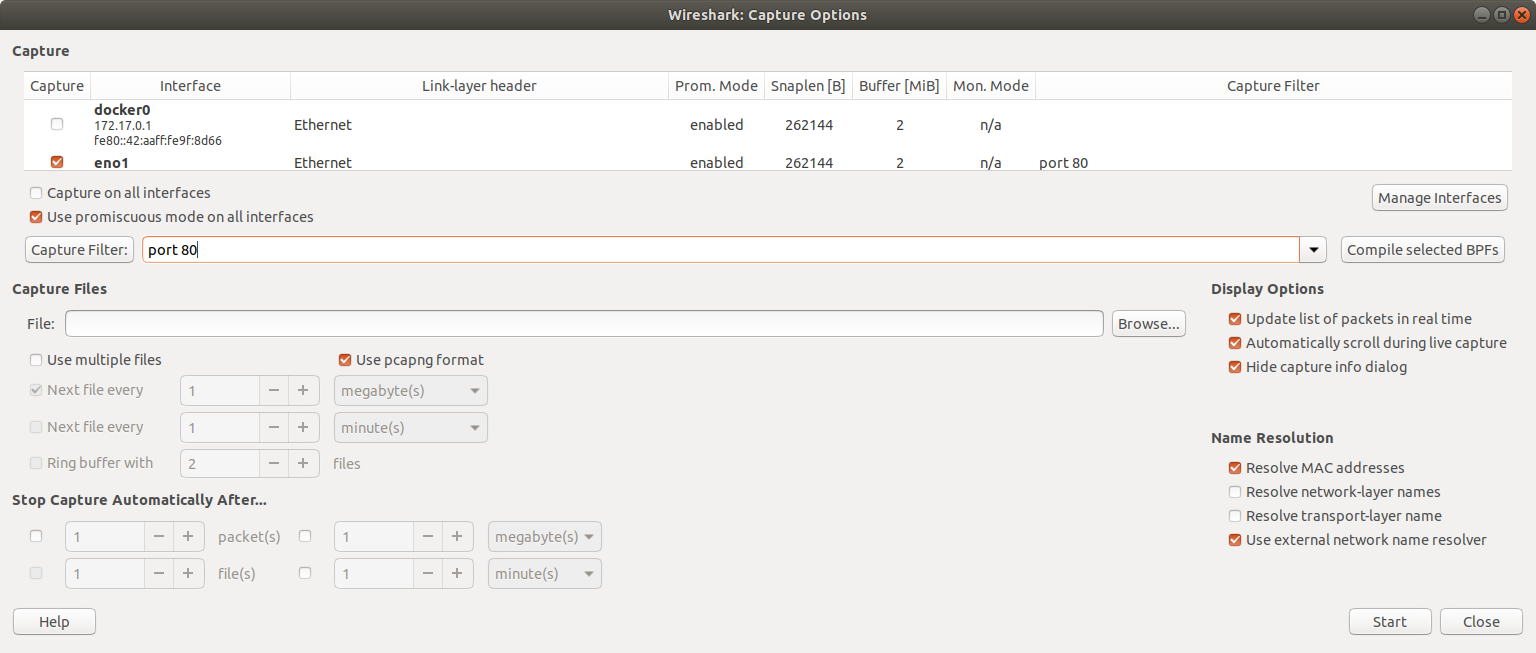
\includegraphics[width=0.7\columnwidth]{\securitydir/WebProtocols/figures/wireshark1.png}
		\par
	\end{centering}
	\caption{\label{fig:wireshark1} Selecting capture filters}
\end{figure}

Then open the browser of your choice and go to the http site chosen. If the configuration of wireshark was successful, you should see the HTTP request we've made to the server and its response. By navigating in the HTTP fields we can gather a lot of information, including browser, OS, and all the headers used
\begin{figure}[htb]
	\begin{centering}
		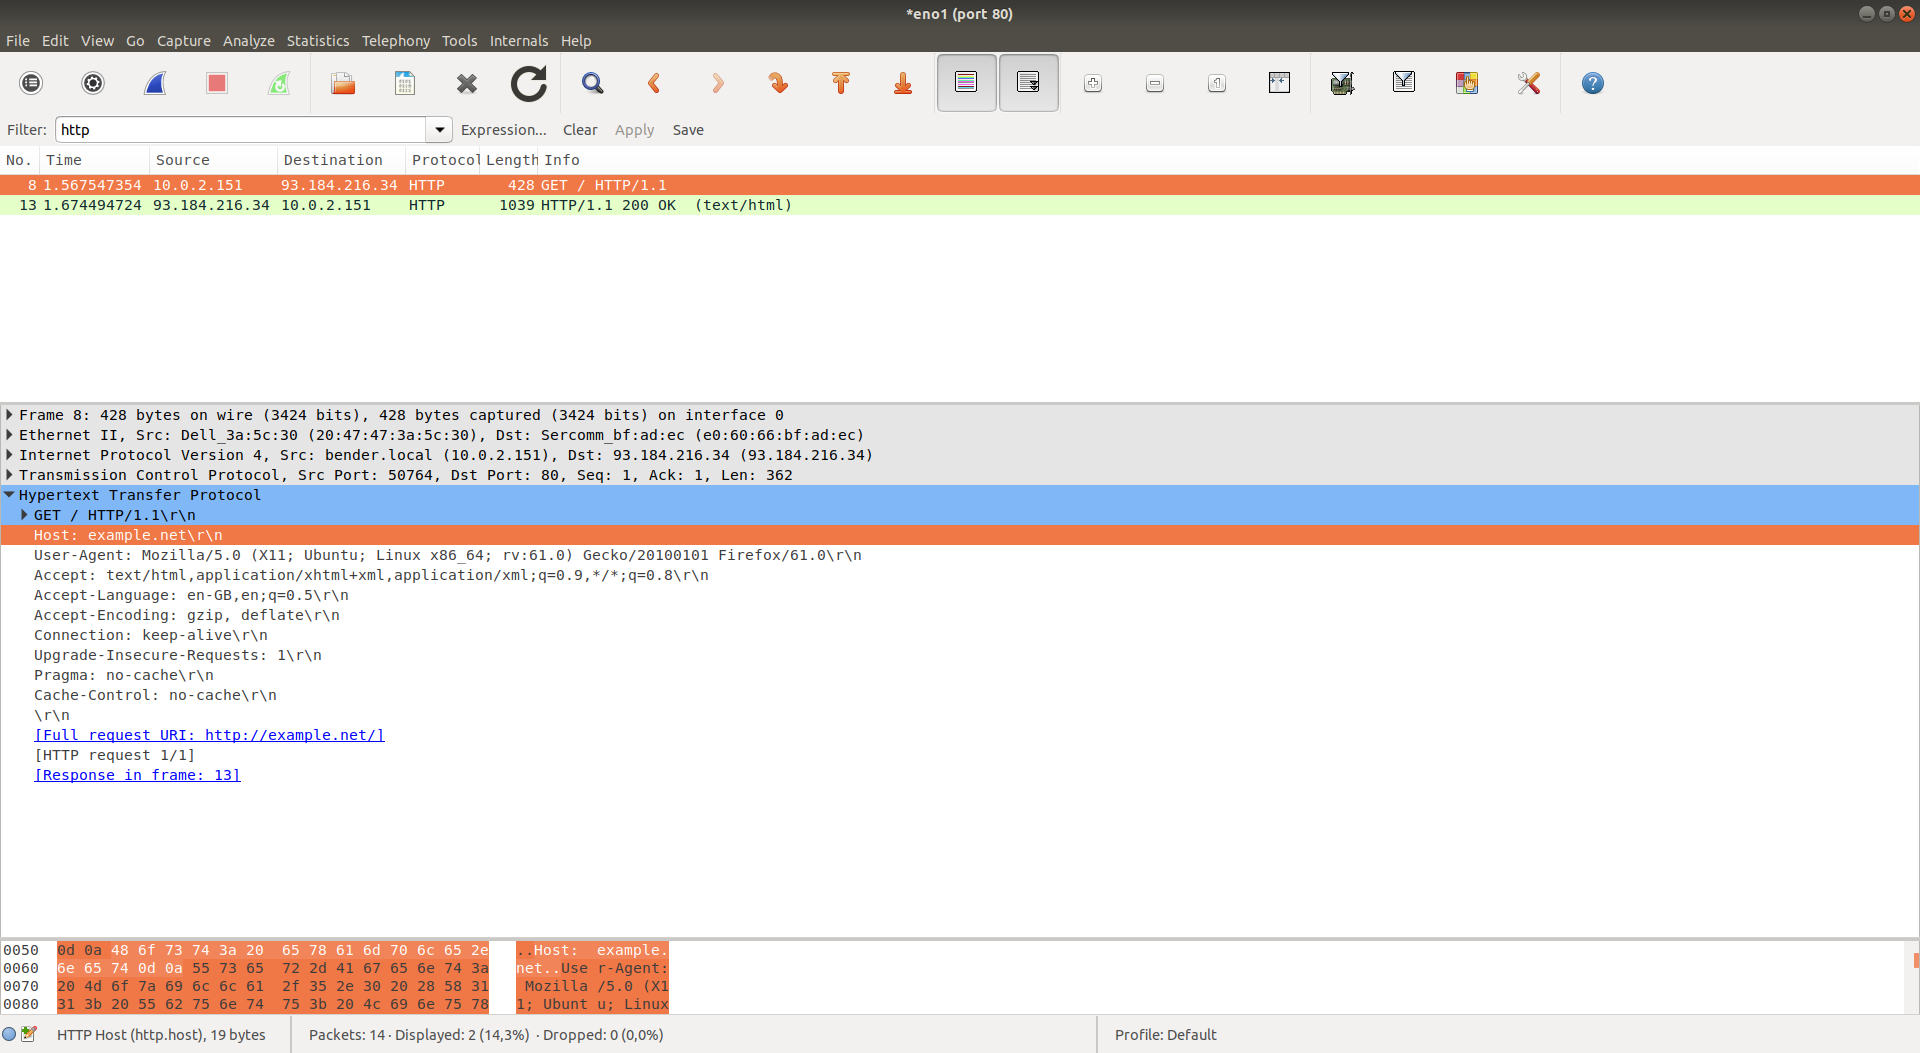
\includegraphics[width=0.7\columnwidth]{\securitydir/WebProtocols/figures/wireshark2.png}
		\par\end{centering}
	\caption{\label{fig:wireshark1} We can see all the fields in a captured request}
\end{figure}

Now we'll gather information on the response made. We can even save the content in a html file and open it with any web browser. To do this, first select the http response and do a left click and then select the option \textbf{Follow HTTP Stream}. 
\begin{figure}[htb]
	\begin{centering}
		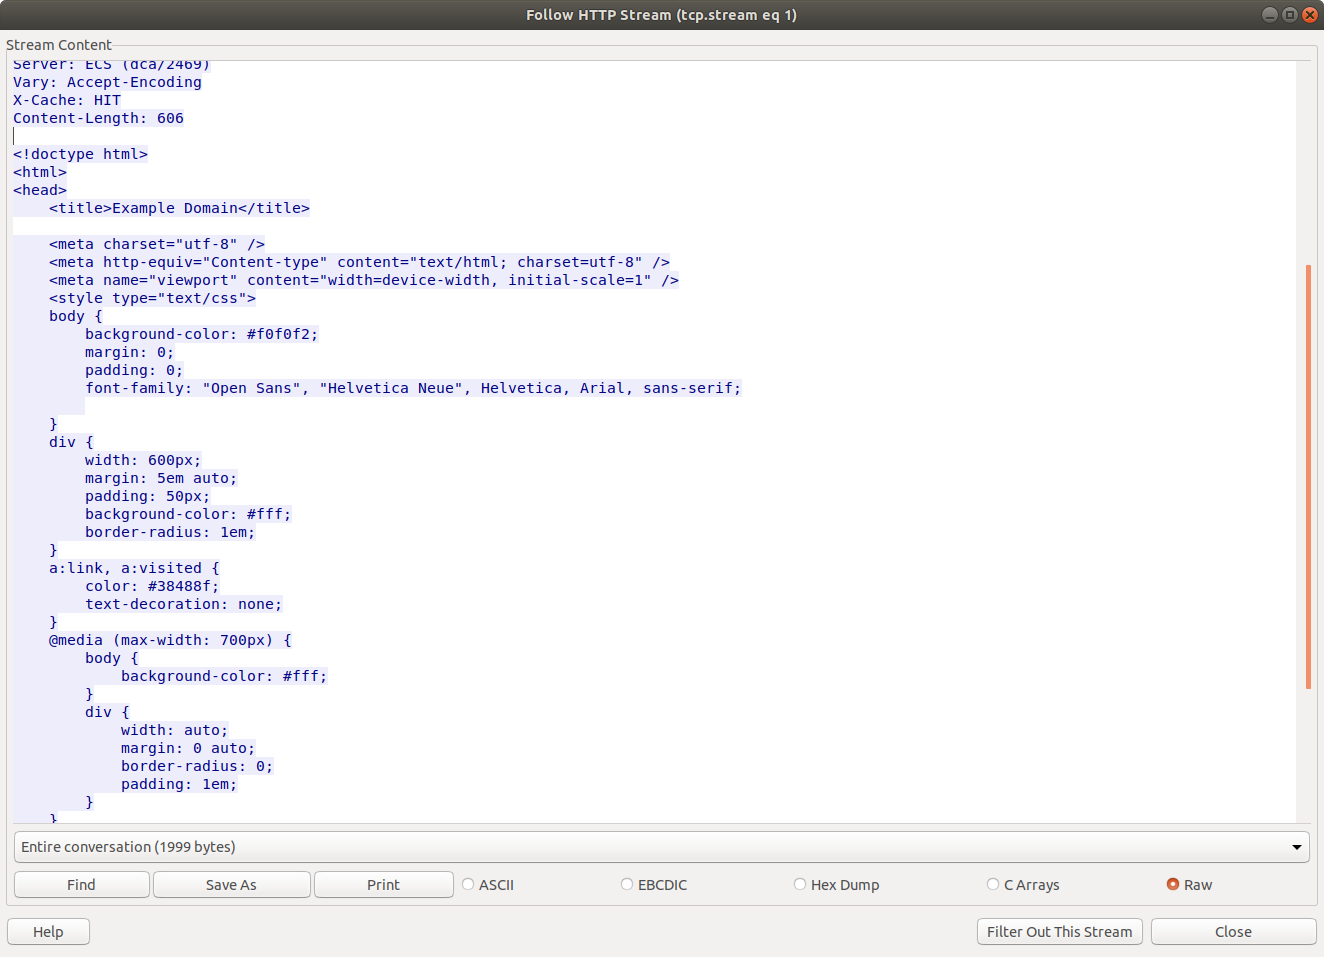
\includegraphics[width=0.7\columnwidth]{\securitydir/WebProtocols/figures/wireshark3.png}
		\par\end{centering}
	\caption{\label{fig:wireshark1} The HTML contained in the response}
\end{figure}
Select the blue text that corresponds to the server response, paste it into the notepad and remove the HTTP headers, leaving only the HTML. Save the file with a .html extension, and then open it using a web browser.
\begin{figure}[htb]
	\begin{centering}
		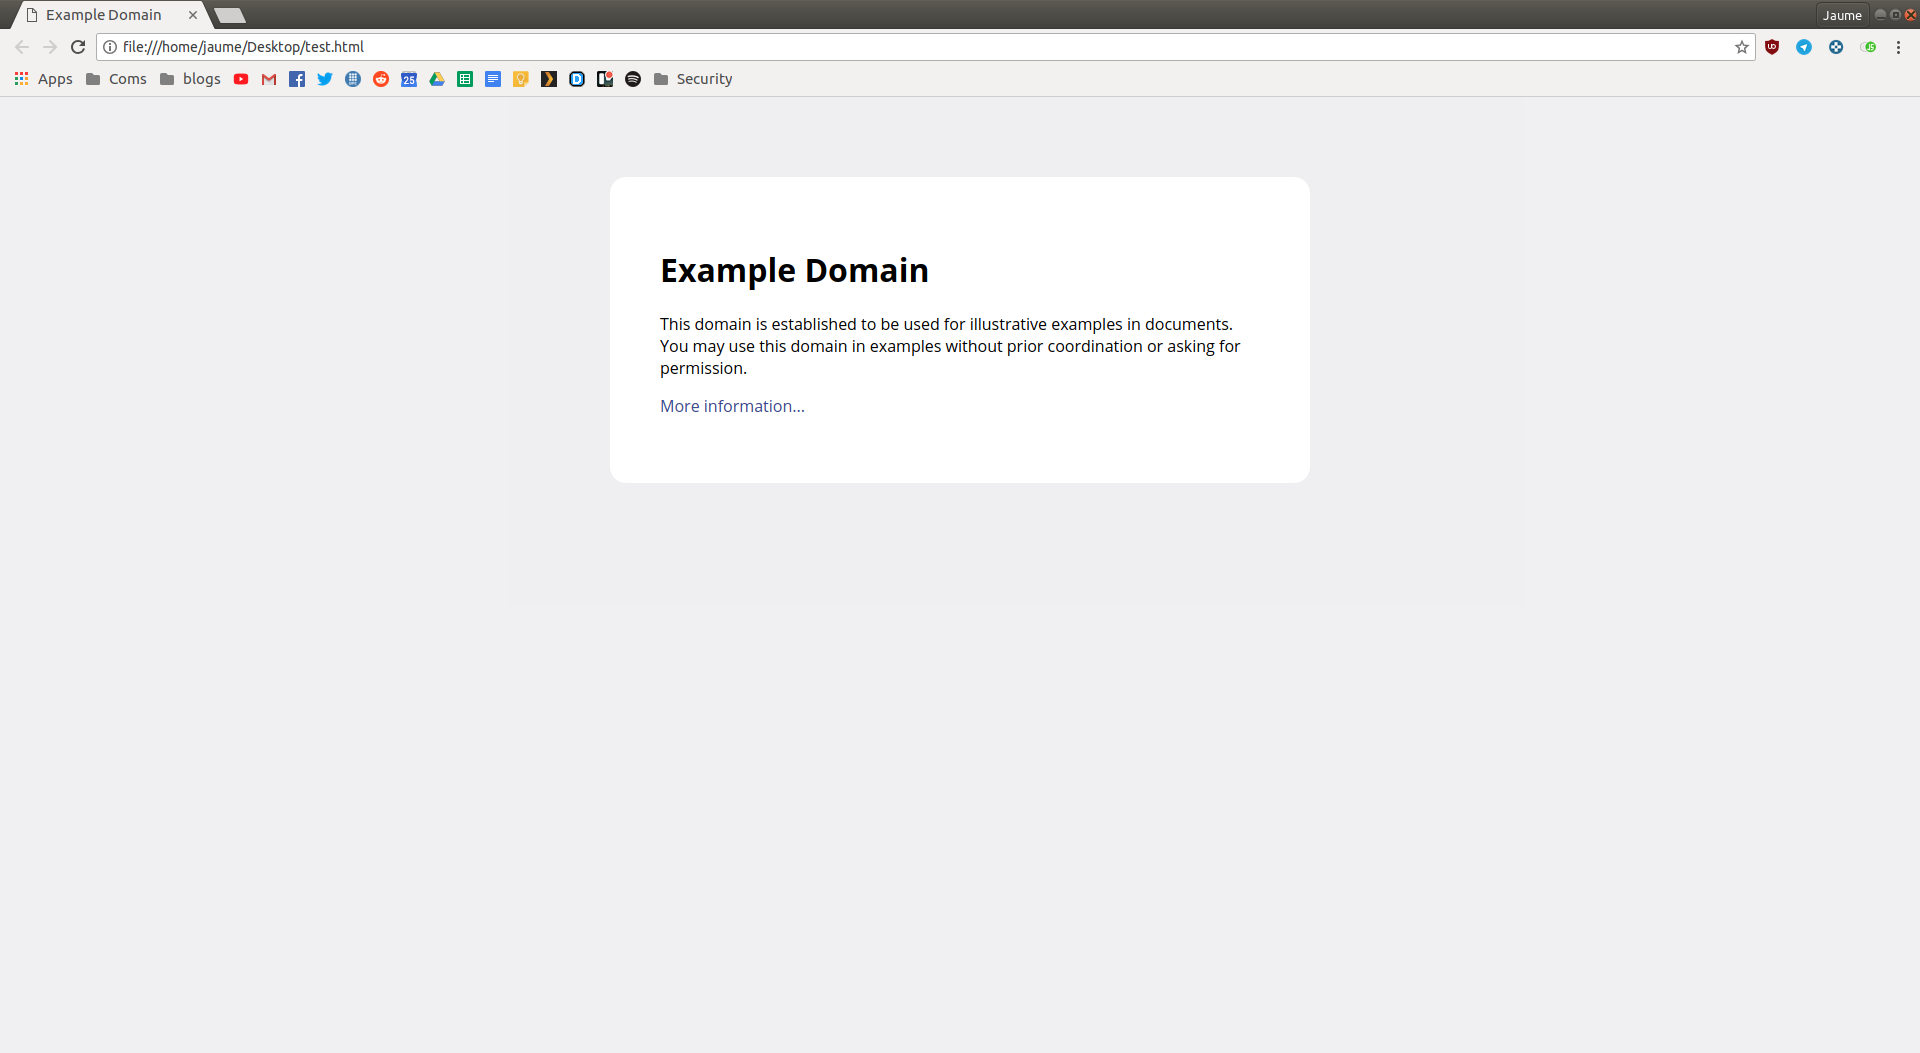
\includegraphics[width=0.7\columnwidth]{\securitydir/WebProtocols/figures/wireshark4.png}
		\par\end{centering}
	\caption{\label{fig:wireshark1} Visualization of the HTML}
\end{figure}

\end{Exercise}

\begin{Answer}[ref={webprotocols-http-practs}]
\end{Answer}

If HSTS was enabled on this domain, the browser would refuse to connect 